\section{生命周期}
在之前的所有权一节,有这么一个函数示例:
\begin{code-block}{rust}
fn first_word(s: &str) -> &str {
    return &s[..];
}

fn copy_ref(s: &str) -> &str {
    // 也可以是&s,为啥?
    return s;
}
\end{code-block}
上述的函数都运行正常。对函数进行改造,改造成下列的样式:
\begin{code-block}{rust}
fn longest(x: &str, y: &str) -> &str {
    if x.len() > y.len() {
        x
    } else {
        y
    }
}
\end{code-block}
即,返回2个字符串当中最长的。如果对这样的代码进行编译,则会出现错误:
\begin{figure}[H]
  \centering
  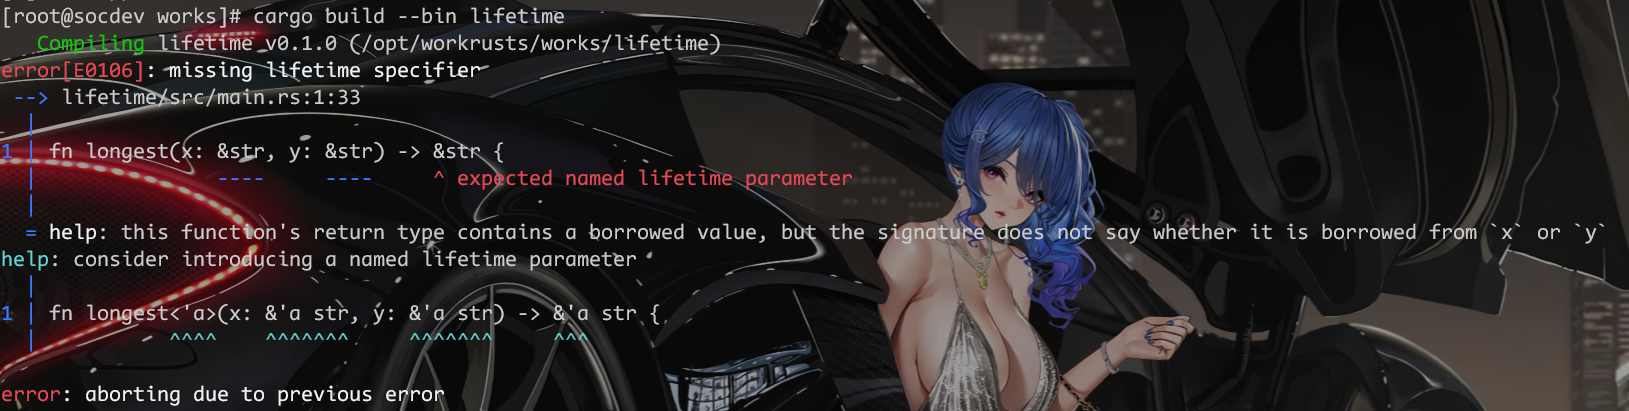
\includegraphics[scale=0.2]{rust_strref_err.png}
  \caption{试图返回多个引用当中的某一个}
  \label{fig:rust_strref_err}
\end{figure}
错误表示,函数应该返回一个有生命周期的命名变量。错误的原因是,Rust编译器无法知道
函数返回的到底是x还是y的引用,无法确定对应的变量的生命周期。

Rust当中,针对引用和借用,有一个特殊的机制:借用检查器,其作用比较作用域来确保所
有的借用都是有效的。
\begin{code-block}{rust}
{
    let r;                      // ---------+-- 'a
    {                            //          |
        let x = 5;             // -+-- 'b  |
        r = &x;                 //  |       |
    }                            // -+       |
    println!("r: {}", r); // ---------+
}
\end{code-block}

其中'a表示变量r原本的作用域(生命周期),'b则表示变量x的有效作用域。进入'b作用域
之后,r变量引用了一个作用域为'b的变量x,当退出'b之后,x失去作用,导致作为x的引用
的r也失去作用,被回收,因此,上述代码无法进行编译:'b的作用范围比'a要小。

为了解决这类的问题,Rust引入了生命周期的操作。生命周期的定义通常使用'+名称的方式
进行定义,表示一个变量或者函数的有效范围,如下:
\begin{code-block}{rust}
&i32        // 引用
&'a i32     // 带有显式生命周期的引用
&'a mut i32 // 带有显式生命周期的可变引用
\end{code-block}
生命周期不仅可以用于变量,同样可以作用与函数和方法上:
\begin{code-block}{rust}
fn main() {
    let string1 = String::from("abcd");
    let string2 = "xyz";

    let res = longest(&string1, string2);
    println!("The result is {}", res);
    println!("The result is {}", res);
}

fn longest<'a>(x: &'a str, y: &'a str) -> &'a str {
    if x.len() > y.len() {
        x
    } else {
        y
    }
}
\end{code-block}
上述代码表示,参数列表当中的所有引用都必须拥有相同的生命周期'a,通过生命周期的限定,
上述代码可以正常编译,并且正常执行。需要注意,如果在参数上使用生命周期,则函数/方法
的前面,则必须加上生命周期,否则会提示参数列表当中的生命周期没有定义。

生命周期同样可以应用于结构体字段定义当中,如下:
\begin{code-block}{rust}
struct ImportantExcerpt<'a> {
    part: &'a str,
}
\end{code-block}

上述结构体的初始化,则可以直接使用字符串的引用进行实现:
\begin{code-block}{rust}
let i = ImportantExcerpt { part: "zhangjl" };
println!("{}", i.part);
\end{code-block}

对于带有生命周期的结构体,在使用的时候,尤其是函数定义和方法定义时,有一些必须
注意的细节:
\begin{outline}[enumerate]
\1 传入外部引用数据模式

使用这种模式,通常情况下,不需要对函数添加生命周期,和普通函数相同。不过,也可以
使用添加生命周期的完整形式:
\begin{code-in-enumerate}{rust}
fn init_struct(source: &str) -> ImportantExcerpt {
    return ImportantExcerpt { part: source };
}

// 使用生命周期的完整形式,实际上是上述函数的完整签名形式
// fn init_struct<'a>(source: &'a str) -> ImportantExcerpt<'a> {
//     return ImportantExcerpt { part: source };
// }

...

// 调用函数
let b = init_struct("luoyan");
\end{code-in-enumerate}
由于上述代码当中,结构体的变量的有效生命周期和外部引用的相同,因此,可以简化生命
周期的使用。

\1 使用函数局部变量

在这种方式下,由于局部引用变量的作用域有限,返回函数之后就不存在了,因此,必须使用
显式的生命周期,而显式的生命周期使用同样有2种形式:
\begin{code-in-enumerate}{rust}
fn init_struct<'a>() -> ImportantExcerpt<'a> {
    return ImportantExcerpt { part: "luoyan"};
}

// 使用静态生命周期,'static表示静态生命周期,为固定关键字
// fn init_struct() -> ImportantExcerpt<'static> {
//     return ImportantExcerpt { part: "luoyan"};
// }
\end{code-in-enumerate}

\1 实现Trait

包含有引用数据类型的结构体,也可以实现各种标准库的Trait。在实现Trait的时候,也
必须使用生命周期:
\begin{code-in-enumerate}{rust}
// 可替换成下面的代码
// impl<'a> fmt::Display for ImportantExcerpt<'a> {
// static可以替换为_
impl fmt::Display for ImportantExcerpt<'static> {
    fn fmt(&self, f: &mut fmt::Formatter) -> fmt::Result {
        write!(f, "{}", self.part)
    }
}
\end{code-in-enumerate}

\1 添加结构体方法

结构体存在引用数据类型,同样要求结构体的方法在实现时需要进行额外的处理,添加生命
周期的使用,同样的,结构体的方法可以使用命名生命周期,也可以使用固定生命周期:
\begin{code-in-enumerate}{rust}
// 使用命名生命周期的结构体方法声明
impl<'a> ImportantExcerpt<'a> {
    fn show(&self) {
        println!("{}", self.part);
    }

    fn reset(&mut self, other: &'a str) {
        self.part = other;
    }

    fn get(&self) -> &str {
        return self.part;
    }
}

// 使用固定生命周期的结构体方法声明
impl ImportantExcerpt<'static> {
    fn show(&self) {
        println!("{}", self.part);
    }

    fn reset(&mut self, other: &'static str) {
        self.part = other;
    }

    fn get(&self) -> &str {
        return self.part;
    }
}
\end{code-in-enumerate}

\end{outline}

在上述的代码当中,很多地方都使用了'static静态生命周期。这是一种特殊的生命周期,
能够存活于整个程序期间,所有的字符串字面值都拥有'static生命周期。但是,并不是
任何情况都建议使用static生命周期。

由于生命周期和泛型以及Trait都非常类似,不可避免的,有可能会遇到几者合用的的情况,
在使用的时候,需要将生命周期与泛型使用,分割开,并且,生命周期应当放在首位。
\begin{code-block}{rust}
fn longest_with_an_announcement<'a, T>(x: &'a str, y: &'a str, ann: T) -> &'a str
    where T: Display
{
    println!("Announcement! {}", ann);
    if x.len() > y.len() {
        x
    } else {
        y
    }
}
\end{code-block}

\section{测试}
Rust的测试与其他语言相同,分为单元测试和集成测试。但不管是单元测试,还是集成测试,
在测试当中,都需要遵循相同的测试规则。在默认的lib类型的crate当中,默认情况下,自动
生成的lib.rs会生成如下的代码:
\begin{code-block}{rust}
#[cfg(test)]
mod tests {
    #[test]
    fn it_works() {
        assert_eq!(2 + 2, 4);
    }
}
\end{code-block}
其中,\#[cfg(test)]表示这是一个测试模块,而\#[test]则表示接下来的函数或者方法是测试
函数,it\_works表示测试的函数/方法名,可以变更为其他的名称。其中,assert!、assert\_eq!
和assert\_ne!这3个宏定义,用于检测运行结果、是否相等/是否不等,比如检测返回值当中
是否包含特定的字符串:
\begin{code-block}{rust}
pub fn greeting(name: &str) -> String {
    format!("Hello {}!", name)
}

#[cfg(test)]
mod tests {
    // 引用暴露的模块代码
    use super::*;

    #[test]
    fn greeting_contains_name() {
        let result = greeting("Carol");
        assert!(result.contains("Carol"));
    }
}
\end{code-block}

如果需要测试panic的代码,则可以使用should\_panic宏进行,该宏表示期望对应的函数在
运行的时候出现panic:
\begin{code-block}{rust}
pub struct Guess {
    value: i32,
}

impl Guess {
    pub fn new(value: i32) -> Guess {
        if value < 1 || value > 100 {
            panic!("Guess value must be between 1 and 100, got {}.", value);
        }

        Guess {
            value
        }
    }
}

#[cfg(test)]
mod tests {
    use super::*;

    #[test]
    #[should_panic]
    fn greater_than_100() {
        Guess::new(200);
    }
}
\end{code-block}
如果测试失败,想在测试结果当中,提示出具体的测试错误信息,则可以添加should\_panic
属性中的expected参数:
\begin{code-block}{rust}
#[cfg(test)]
mod tests {
    use super::*;

    #[test]
    #[should_panic(expected = "Guess value must be between 1 and 100")]
    fn greater_than_100() {
        Guess::new(200);
    }
}
\end{code-block}

运行测试用例时,只需要简单的输入如下的指令即可:
\begin{code-block}{bash}
// 默认并行的方式运行所有的测试用例
cargo test

// 串行的方式运行所有的测试用例
cargo test -- --test-threads=1

// 运行指定的测试用例,可匹配以add开头的所有测试用例
cargo test add
\end{code-block}

需要单独说明的是Rust的集成测试。集成测试通常针对lib型的crate。其测试过程大致如下:
\begin{outline}[enumerate]
\1 创建一个lib,并编写代码

\begin{code-in-enumerate}{bash}
cargo new --lib shared
\end{code-in-enumerate}

\1 在shared的src同级目录下,创建集成测试用例目录:
\begin{code-in-enumerate}{bash}
# 文件夹名称固定为tests
mkdir tests
\end{code-in-enumerate}

\1 在tests下创建集成测试用例
\begin{code-in-enumerate}{bash}
echo > tests/units.rs<<EOF
// 导入的lib名称必须是当前crate的名称
use shared;

#[test]
fn it_adds_two() {
    assert_eq!(4, adder::add_two(2));
}
EOF
\end{code-in-enumerate}
然后执行测试即可。
\end{outline}

\section{Rust的函数式编程}
Rust同样支持函数式编程。相比于其他语言,Rust的函数式编程性能和效率更高。Rust常见的
函数式编程模式包括闭包和迭代器2大类。

\subsection{闭包}
Rust的闭包和Python当中的非常类似,都可以直接读取外部的变量。其定义的形式基本如下:
\begin{code-block}{rust}
let expensive_closure = |num| {
    println!("calculating slowly...");
    num * 10
};

let res = expensive_closure(10);
\end{code-block}
其中两个||表示定义一个闭包,中间的num表示闭包的参数。如果闭包需要处理多个参数,则
应该改写为:
\begin{code-block}{rust}
let expensive_closure = |num1, num2| {
    num1 * num2
};
\end{code-block}

从实际的使用当中可以看到,Rust的闭包实际上就是一个匿名函数,在Rust当中,函数都有
参数类型/返回值的声明,但是,在上述的代码当中,却没有看到相关的定义和声明。这是
因为Rust的闭包通常很短,并只关联于小范围的上下文而非任意情境。在这些有限制的上下
文中,编译器有能力可靠的推断参数和返回值的类型,如同能够推断大部分变量的类型一样。
不过,不注明参数/返回类型,有可能出现一种迷惑性的使用:即无法传入正确的数据类型,
如下:
\begin{code-block}{rust}
let example_closure = |x| x;

let s = example_closure(String::from("hello"));
let n = example_closure(5);
\end{code-block}
按照上述代码的定义,example\_closure只是将输入参数原封不动的返回给调用者,第1次
调用时,编译器会将该闭包推断为输入/输出为字符串类型,然后这些类型信息会被锁定到
该闭包当中。后续再传入数值,由于闭包的类型已经锁定,要求传入字符串,但实际传入的
是数值,结果就会导致上述代码出现错误:
\begin{figure}[H]
  \centering
  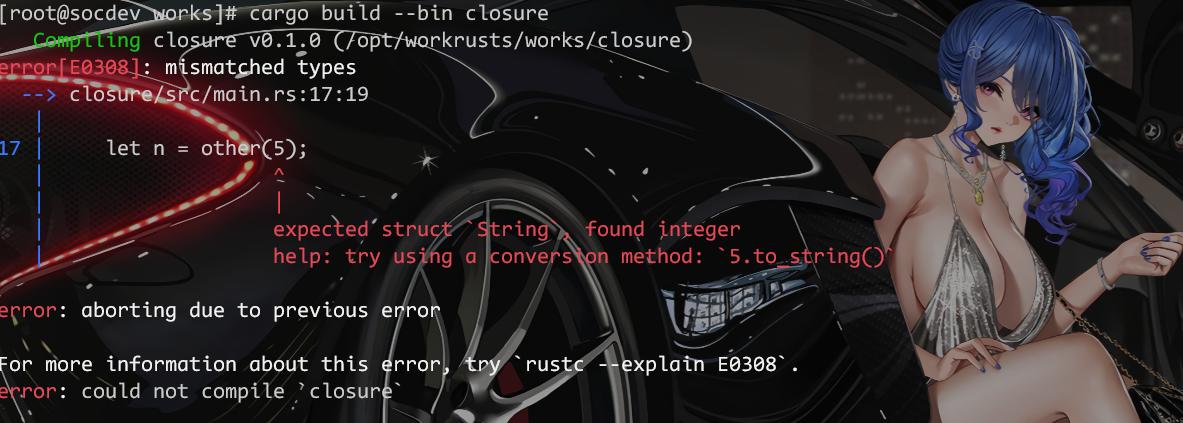
\includegraphics[width=\linewidth]{rust_closure_diffrent_type.png}
  \caption{试图处理不同数据类型的闭包}
  \label{fig:rust_closure_diffrent}
\end{figure}

闭包的完整定义(包括类型)则如下:
\begin{code-block}{rust}
let live_closure = |num: i32| -> (i32, i32) {
    println!("calculating slowly...");
    thread::sleep(Duration::from_secs(2));
    (num * 10, num * 20)
    // 或者修改为return语句
    // return (num*10, num*20);
};

// 如果不需要返回值,则闭包的写法需要注意一下:
let other = |x| {
    println!("{}", x);
};
\end{code-block}

\subsection{特殊的闭包}
默认的情况下,包括Python和Golang,闭包都只是匿名函数。不过,在Rust当中,闭包可以
用在结构体当中,其主要用途就是memoization或lazy evaluation(惰性求值),即懒加载。
当结构体当中存放闭包时,则必须注明闭包的类型。而在结构体/枚举当中使用闭包,则需要
使用trait和泛型:Fn、FnMut和FnOnce。这3者的区别如下:
\begin{enumerate}
  \item FnOnce:闭包内对外部变量存在转移操作,导致外部变量不可用,所以只能call一次
  \item FnMut:闭包内对外部变量直接使用,并进行修改
  \item Fn:闭包内对外部变量直接使用,不进行修改
\end{enumerate}

使用这些trait的时候,则必须注明闭包的参数/返回值的类型。比如,闭包接收一个u32的
参数,返回一个u32,则对应的Fn trait bound则如下:
\begin{code-block}{rust}
Fn(u32) -> u32
\end{code-block}

一个包含闭包的结构体示例如下:
\begin{code-block}{rust}
struct Cacher<T>
where
    T: Fn(u32) -> u32,
{
    calculation: T,
    value: Option<u32>,
}
\end{code-block}
对该结构体的解读如下:结构体Cacher包含一个泛型calculation,而这个泛型则是一个使用
了Fn的闭包,这个闭包接收一个u32的参数,并最终返回一个u32。Value则是用于存放calculation
的计算结果,便于第二次调用时,直接返回而无需计算。根据上述需求,整个结构体的方法
实现如下:
\begin{code-block}{rust}
impl<T> Cacher<T>
where
    T: Fn(u32) -> u32,
{
    pub fn new(calculation: T) -> Cacher<T> {
        Cacher {
            calculation: calculation,
            value: None,
        }
    }

    pub fn value(&mut self, arg: u32) -> u32 {
        match self.value {
            Some(v) => v,
            None => {
                let v = (self.calculation)(arg);
                self.value = Some(v);
                v
            }
        }
    }
}
\end{code-block}
注意,在上述的结构体以及结构体方法当中,首次出现了trait bound和where的使用。需要
特别说明事实,trait bound几乎可以用于Rust的任何场景。New方法接收一个泛型作为初始化
参数,这个泛型就是一个Fn的闭包;而value方法则是根据根据当前结构体的数据,直接进行
数据的返回,或者计算,再返回。该结构体的使用方式如下:
\begin{code-block}{rust}
let mut cacher = Cacher::new(|x: u32| -> u32 { x * 10 });
let mut val = cacher.value(32);
println!("The val of cacher is {}", val);

val = cacher.value(45);
println!("The val of cacher second time is {}", val);
\end{code-block}
只是稍微可惜的是,这个表示缓存的结构体还存在bug,2次传入不同的数据,却得到了相同的
结果。问题在于字段value的定义。可以考虑使用Hashmap或者其他数据类型来替换value。一种
可能的解决方法如下:
\begin{code-block}{rust}
struct Cacher<T>
where
    T: Fn(u32) -> u32,
{
    calculation: T,
    value: BTreeMap<u32, Option<u32>>,
}

impl<T> Cacher<T>
where
    T: Fn(u32) -> u32,
{
    pub fn new(calculation: T) -> Cacher<T> {
        Cacher {
            calculation: calculation,
            value: BTreeMap::new(),
        }
    }

    pub fn value(&mut self, arg: u32) -> u32 {
        // 从现有的结果记录当中查询是否存在arg对应的计算结果
        match self.value.get(&arg) {
            // 找到则直接返回
            Some(Some(x)) => *x,
            // 没有找到,则计算一次,并放入当前的结果集合
            Some(None) | None => {
                let v = (self.calculation)(arg);
                self.value.insert(arg, Some(v));
                v
            }
        }
    }
}
\end{code-block}

闭包同样可以捕获运行环境的上下文,即在闭包内部直接使用外部的所有变量:
\begin{code-block}{rust}
fn main() {
    let x = 4;
    let equal_to_x = |z| z == x;
    let y = 4;
    assert!(equal_to_x(y));
}
\end{code-block}
X在闭包出现之前已经存在,定义闭包equal\_to\_x的时候,可以直接使用外部的x,而无需
重新声明。

\subsection{迭代器}
迭代器是Rust函数式编程的另外一个利器,负责遍历序列中的每一项和决定序列何时结束的
逻辑,我们在使用的时候,就无需判断开始条件和结束条件。在Rust当中,迭代器是惰性的,
只有使用到了,才会在内存当中进行展开。Rust的迭代器必须实现一个Iterator的triat,
这个trait的定义类似如下的结构:
\begin{code-block}{rust}
pub trait Iterator {
    type Item;
    fn next(&mut self) -> Option<Self::Item>;
    ...
}
\end{code-block}
其中的type Item和Self::Item定义了trait的关联数据类型,即该trait要求同时定义一个
Item类型,该类型被用作next方法的返回值类型。Next方法是Iterator被要求实现的唯一
方法,其一次返回一个项,最后返回一个None。

Rust的next方法得到的是迭代器的不可变引用,iter方法生成一个不可变引用的迭代器。
如果我们需要一个获取所有权并返回拥有所有权的迭代器,则可以调用into\_iter而不是iter。
类似的,如果我们希望迭代可变引用,则可以调用iter\_mut而不是iter;如果一旦调用了
into\_iter,则迭代完成之后,迭代器不再有效,比如下方代码:
\begin{code-block}{rust}
let v = vec![1, 2, 3];
let v3: Vec<_> = v.into_iter().map(|x| x * 12).collect();
println!("{:?}", v3);
println!("{:?}", v);
\end{code-block}
一旦进行编译,则会提示如下的错误:
\begin{figure}[H]
  \centering
  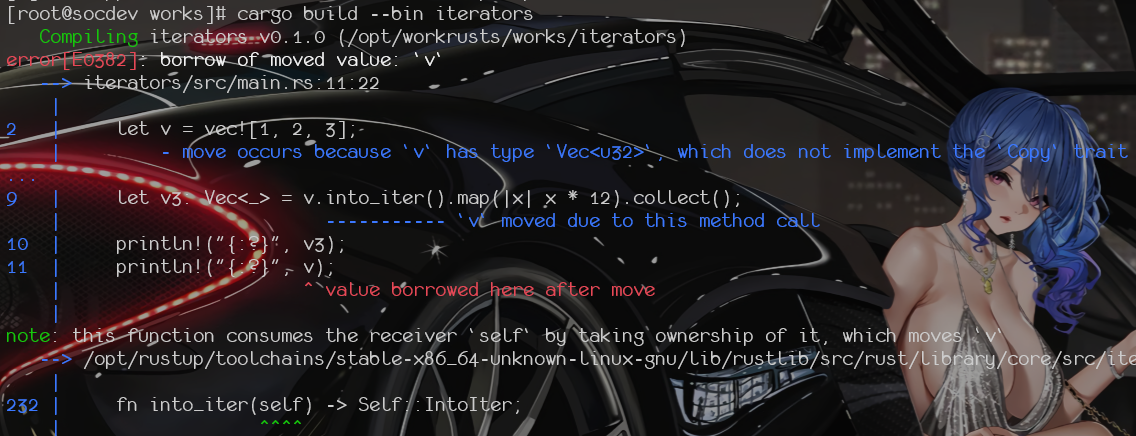
\includegraphics[width=\linewidth]{rust_iter_move.png}
  \caption{迭代器的所有权转移}
  \label{fig:rust_iter_move}
\end{figure}

实际上,上述的操作相当于对一个迭代器进行了消费。一般说来,调用next方法的方法被称为
消费适配器(consuming adaptors),因为调用他们会消耗迭代器。一个消费适配器的例子
是sum方法。这个方法获取迭代器的所有权并反复调用next来遍历迭代器,因而会消费迭代器。
当其遍历每一个项时,它将每一个项加总到一个总和并在迭代完成时返回总和。在这个过程
完成之后,原有的迭代器将无法再继续使用,因为其所有权已经进行了转移。
\begin{code-block}{rust}
let v = vec![1, 2, 3];
let v_item = v.iter();
let total1: u32 = v_item.sum();
// 迭代器v_item不再有效
println!("{:?}", v_item);
\end{code-block}

Iterator trait中定义了另一类方法,被称为迭代器适配器(iterator adaptors),允许
我们将当前迭代器变为不同类型的迭代器,并且可以链式调用多个迭代器适配器。不过因为
所有的迭代器都是惰性的,必须调用一个消费适配器方法以便获取迭代器适配器调用的结果。
比较常见的,就是使用map函数(迭代适配器,遍历迭代器的所有元素)来生成新的迭代器。
与之相对应的,collect方法则是消费迭代器并将结果收集到一个数据结构中。同样需要注意
的是,任何的迭代消费器,都不能进行类型的自动推导,需要手动的指定对应的数据类型。
比如,sum的结果通常是数值类型,而collect的结果则通常是vec类型。

迭代器和闭包通常结合使用,因为闭包可以捕获环境,比如常用的filter迭代器适配器:
\begin{code-block}{rust}
let v = vec![1, 2, 3];
// 使用的是iter,即引用数据类型,但是filter使用的本身是引用,因此,需要进行
// 2次的解引用操作
let res: Vec<_> = v.iter().filter(|s| *(*s) == 2).collect();
println!("{:?}", res);
// 原始的v仍然可用,没有发生所有权转移
println!("{:?}", v);

// 发生了所有权转移,变量v在后续的操作当中,无法被继续使用
let res1: Vec<_> = v.into_iter().filter(|s| *s == 2).collect();
println!("{:?}", res1);
\end{code-block}

Filter和迭代器使用的时候,需要特别注意所有权以及引用数据类型,特别是复合数据类型。
不同的操作会导致复合数据类型的所有权的变更。
\begin{code-block}{rust}
struct Shoe {
    size: u32,
    style: String,
}

fn main() {
    let shoes = vec![
        Shoe {
            size: 10,
            style: String::from("sneaker"),
        },
        Shoe {
            size: 13,
            style: String::from("sandal"),
        },
        Shoe {
            size: 10,
            style: String::from("boot"),
        },
    ];

    // 正确,返回的结果r实际上是shoes的部分数据的引用
    let r: Vec<_> = shoes.iter().filter(|x| x.size == 10).collect();

    // 错误,无法编译,由于collect返回的是引用,无法直接转换成引用原本的数据类型
    let r1: Vec<Shoes> = shoes.iter().filter(|x| x.size == 10).collect();

    // 正确,使用into_iter获取了相关的所有权,不再是引用,而是原始数据类型
    let r2: Vec<Shoes> = shoes.into_iter().filter(|x| x.size == 10).collect();
    // 在此之后,shoes变量无法再使用,所有权已经发生了变更

    // 错误,shoes的所有权已经发生了变更,此处已经无效
    shoes_in_my_size(shoes, 10);
}

// 调用者发生了所有权转移,调用该函数之后,参数shoes无法再被使用
fn shoes_in_my_size(shoes: Vec<Shoe>, shoe_size: u32) -> Vec<Shoe> {
    shoes.into_iter().filter(|s| s.size == shoe_size).collect()
}
\end{code-block}

\subsection{自定义迭代器}
可以通过在vector上调用iter、into\_iter或iter\_mut来创建一个迭代器,也可以用标准库
中其他的集合类型创建迭代器,比如哈希map。另外,可以实现Iterator trait来创建任何
我们希望的迭代器,如下:
\begin{code-block}{rust}
impl Counter {
    fn new(max: u32) -> Counter {
        return Counter {
            current: 0,
            max: max,
        };
    }
}

impl Iterator for Counter {
    type Item = u32;
    fn next(&mut self) -> Option<Self::Item> {
        self.current += 1;

        if self.current <= self.max {
            Some(self.current)
        } else {
            None
        }
    }
}
\end{code-block}
然后,即可像普通的集合数据类型Vec一样,使用for和next进行操作:
\begin{code-block}{rust}
let c = Counter::new(10);

// 忽略开头的n个数据
// for item in c.skip(1) {
// 像迭代器一样的使用类型
for item in c {
   println!("{}", item);
}

// 需要注意,c的所有权已经被转移,在此之后,无法再使用变量c

let c1 = Counter::new(10);
let c2 = Counter::new(20);

let sum: u32 = c1
    .zip(c2.skip(10))
    .map(|(a, b)| a * b)
    .filter(|x| x % 3 == 0)
    .sum();
println!("{}", sum);
\end{code-block}
上述的自定义迭代器并不完整,比如,默认情况下转移了变量的所有权,无法使用变量的引用
进行迭代等等。这些问题可以在后续进行进一步的改进。

\section{智能指针}
Rust当中同样存在指针,最常用的指针就包括引用数据类型。除了引用数据之外,引用类型
没有其他任何特殊的操作,也不存在其他额外的开销。除此之外,Rust还拥有智能指针,
这是一种数据结构,其表现类似于真正的指针,但是,拥有额外的元数据和功能。普通的引用
只是借用数据,而智能指针则是拥有指向的数据。

常见的智能指针包括String以及Vec<T>,通常使用结构体实现。和普通结构体明显区别的是,
智能指针实现了Deref和Drop这2个trait。Deref trait允许智能指针结构体实例表现的像引
用一样,这样就可以编写既用于引用、又用于智能指针的代码;Drop trait允许我们自定义
当智能指针离开作用域时运行的代码。在标准库当中最常用的智能指针主要包含下列3种:
\begin{enumerate}
  \item Box<T>:用于在堆上分配值
  \item Rc<T>:引用计数类型,其数据可以有多个所有者
  \item Ref<T> 和 RefMut<T>:通过RefCell<T>访问,RefCell<T>是一个在运行时而不是在编译时执行借用规则的类型
\end{enumerate}

\subsection{使用Box指向内存堆上的数据}
最简单直接的智能指针是box,其类型是 Box<T>。Box允许你将一个值放在堆上而不是栈上,
留在栈上的则是指向堆数据的指针。相比于普通的变量,Box的数据存放在内存堆上,但是
没有任何的性能损失,通常用于下列的场景当中:
\begin{itemize}
\item 当有一个在编译时未知大小的类型,而又想要在需要确切大小的上下文中使用这个类型值的时候
\item 当有大量数据并希望在确保数据不被拷贝的情况下转移所有权的时候
\item 当希望拥有一个值并只关心它的类型是否实现了特定trait而不是其具体类型的时候
\end{itemize}

第一种情况通常用于递归数据类型;第二种情况,转移大量数据的所有权会消耗大量的时间,
通过box将数据放在内存堆上,只有少量的指针数据在栈上被拷贝,减小了时间消耗;第三种
情况则通常称之为trait对象。

使用Box分配和使用堆上的数据示例如下:
\begin{code-block}{rust}
let v = Box::new(5);
let s = 10;

// Box类型无法直接和其他数据类型进行计算,必须进行转换
// 在本例当中,v的数据类型为Box<{integer}>
let b = v.as_ref() + s;
// 或者修改为如下的方式
// let b = *v + s;

println!("{}", b);
println!("{}", v);
\end{code-block}

Rust编译器要求在编译期间就能够确定对应的类型所占用的存储空间,但是,Rust当中也
存在无法在编译期间明确大小的数据类型,即递归数据类型。这种特殊类型的值,可以是
相同类型的另一个值,并且,这种嵌套关系可以无限进行下去,因此,Rust是不知道递归
数据类型的存储空间的。但是,可以通过在递归类型当中插入Box,以此为基准进行递归
数据类型的创建。

递归数据类型是一种特殊的数据类型,来源于Lisp,常见的开发语言当中没有与之相对的,
一个简单的递归数据类型的定义如下:
\begin{code-block}{rust}
enum List {
    Cons(i32, List),
    Nil,
}
\end{code-block}
Cons由2部分组成:自己包含的数据i32和另外一个List对象,其最后一项值包含一个叫做Nil
的值且没有下一项,代表递归的终止条件就是Nil。可以明显的看到,该数据类型理论上可
以无限的递归循环下去,我们无法在编译阶段就明确其存储空间占据的大小,因此上述代码
目前还无法编译通过。为了使得上述代码成功编译,可以利用Box特性:
\begin{code-block}{rust}
#[derive(Debug)]
enum List {
    Cons(i32, Box<List>),
    Nil,
}

use crate::List::{Cons, Nil};
fn main() {
    let list = Cons(1, Box::new(Cons(2, Box::new(Cons(3, Box::new(Nil))))));
    println!("{:?}", list);
}
\end{code-block}

通过这样的改变,Cons的大小就确定了:需要存放一个i32大小的值,以及一个Box指针大小
的数据(usize),从内存结构上看,其分布大致如下:
\begin{figure}[H]
  \centering
  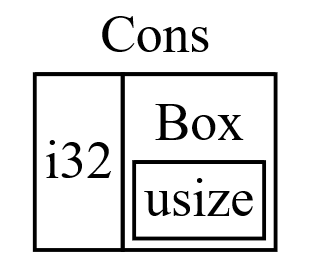
\includegraphics[scale=0.4]{rust_box.png}
  \caption{递归数据类型的内存示意}
  \label{fig:rust_box}
\end{figure}

\subsection{Deref Trait:将智能指针当作常规引用}
Deref Trait允许重载解引用操作符(*),将智能指针当作常规引用。在此之前,先看看
引用和原始数据之间的联系:
\begin{code-block}{rust}
let x = 5;
let y = &x;

// 正确,引用被转换成原始数据类型
let r = y + 9;
println!("{}, {}", y, r );

// 提示错误,代码无法进行编译和运行
println!("{}", y == 5);

// 提示错误,代码无法进行编译和运行
if y > 2 {
    ...
}
// 提示错误,代码无法进行编译和运行
assert_eq!(5, y);

// 正确,通过解引用,将引用变更为对应的类型
assert_eq!(5, y);

let mut yy = &x;
// 错误,无法编译
yy = yy + 10;
\end{code-block}
上述代码看起来是没有错误的,但是在编译的时候,会提示一个错误信息:
\begin{figure}[H]
  \centering
  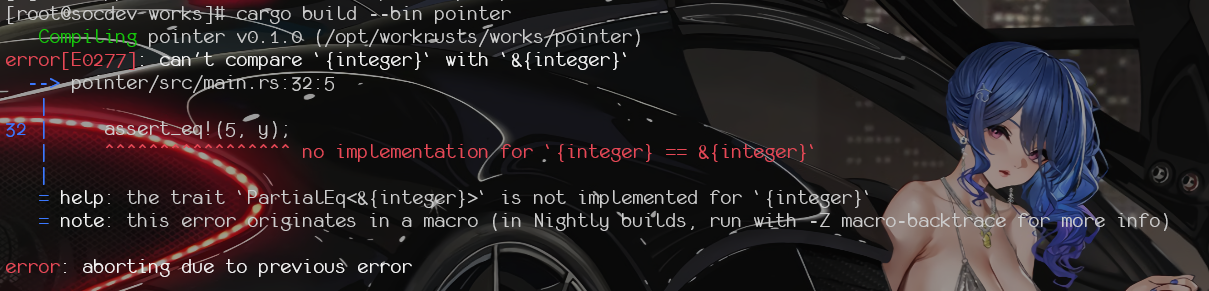
\includegraphics[width=\linewidth]{rust_pointer_error.png}
  \caption{尝试直接进行引用类型和其他类型的比较}
  \label{fig:rust_pointer_error}
\end{figure}
其根本原因在于,y虽然在使用上大多数情况和x没有什么区别,但是,实质上,y是一个引用
数据类型(指针),数值和x是具体的数值类型,引用和数值类型之间无法进行相互的比较。
如果需要进行对比,则需要对y进行解引用操作,或者直接使用原始的x。同样的,引用数据
类型和数值类型进行计算,得到的结果是数值类型,而并非引用数据类型。如果使用Box来替换
引用数据类型,其结果相同:
\begin{code-block}{rust}
let x = 5;
let y = Box::new(x);
// 提示错误,同样是由于数据类型不匹配
assert_eq!(5, y);
// 正确,通过解引用,将引用变更为对应的类型
assert_eq!(5, *y);
\end{code-block}

同样的,可以用Deref Trait实现自定义的智能指针。从本质上讲,Box<T>实际上是一个被
定义为包含一个元素的元组结构体(元组当中只包含一个元素),可以根据这个思路自定义
类似Box的智能指针:
\begin{code-block}{rust}
struct Pointer<T>(T);

impl<T> Pointer<T> {
    fn new(x: T) -> Pointer<T> {
        Pointer(x)
    }
}
\end{code-block}
上述代码使用泛型T作为元组的参数,使得该结构体可以嵌入/使用任何数据类型。接着实现
该结构的Deref Trait:
\begin{code-block}{rust}
impl<T> Deref for Pointer<T> {
    type Target = T; // 定义关联类型
    fn deref(&self) -> &T {
        &self.0
    }
}
\end{code-block}
也就是说,针对智能指针Pointer,已经可以实现对泛型数据的封装,并且可以正常的进行
解引用操作:
\begin{code-block}{rust}
// 代码可以正常的运行
let p = Pointer::new(5);
assert_eq!(5, *p);

let s = Pointer::new("lucifer");
assert_eq!("lucifer", *s);
\end{code-block}

在Rust当中,实现了Deref Trait的数据类型,在使用时,会将其引用转换为原始数据类型,
这种转换通常称之为解引用强制多态。当这种特定类型的引用作为实参传递给和形参类型
不同的函数或方法时,解引用强制多态将自动发生:
\begin{code-block}{rust}
fn hello(name: &str) {
    println!("Hello, {}!", name);
}

fn main() {
    let m = Pointer::new(String::from("Rust"));
    hello(&m);
}
\end{code-block}
上述代码当中,使用\&m调用hello函数,其为Pointer<String>值的引用,因为在Pointer<T>
上实现了Deref trait,Rust可以通过deref调用将Pointer<String>变为\&String,同时标准
库中提供了String上的Deref实现,其会返回字符串slice,Rust再次调用deref将\&String
变为\&str,这就符合hello 函数的定义了。

如果没有解引用强制多态的特性,则函数的调用则必须变更为如下的样式:
\begin{code-block}{rust}
hello(&(*m)[..]);
\end{code-block}
即(*m)将Pointer<String>解引用为String。接着\&和[..]获取了整个String的字符串slice
来匹配hello的签名,这无疑是一种低效的使用方式。

Deref重载的是不可变引用的*运算符,DerefMut则用于重载可变引用的*运算符。当发现如下
的几种情况时,Rust会进行解引用的强制多态:
\begin{itemize}
  \item 当T: Deref<Target=U> 时从\&T到\&U
  \item 当T: DerefMut<Target=U> 时从\&mut T到\&mut U
  \item 当T: Deref<Target=U> 时从\&mut T到\&U
\end{itemize}
第一种情况表明如果有一个\&T,而T实现了返回U类型的Deref,则可以直接得到\&U;第二种
情况表明对于可变引用也有着相同的行为;第3种情况,将可变引用强转为不可变引用,但
反过来是不行的,即不可变引用永远也不能强转为可变引用。

\subsection{使用Drop trait清理}
对于智能指针模式来说第二个重要的trait是Drop,其允许我们在值要离开作用域时执行一
些代码。默认可以为任何类型提供Drop trait的实现,同时所指定的代码被用于释放类似
于文件或网络连接的资源。

在其他一些语言中,我们不得不记住在每次使用完智能指针实例后调用清理内存或资源的代码。
如果忘记的话,运行代码的系统可能会因为负荷过重而崩溃。在Rust中,可以指定每当值离
开作用域时被执行的代码,编译器会自动插入这些代码,不需要在程序中到处编写在实例结
束时清理这些变量的代码,而且还不会出现内存泄漏。

Drop trait比较类似于C++的析构函数,用于指定对应的对象在离开作用域时需要进行的清理
代码,要求实现一个drop函数。简单的示例如下:
\begin{code-block}{rust}
struct SmartPointer {
    data: String,
}

impl Drop for SmartPointer {
    fn drop(&mut self) {
        println!("Drop the smart pointer {}", self.data);
    }
}

fn main() {
    let p = SmartPointer::new("zhangjl");
}
\end{code-block}
虽然在main函数当中,没有执行任何的输出操作,但是当代码结束运行时,还是会打印出
drop函数的执行结果,就如同析构函数一般。但和析构函数不同的是,析构函数可以通过
del操作调用,而Rust的drop函数是无法调用或者禁用的。如果需要提前释放变量,则需要
使用std::mem::drop进行替换:
\begin{code-block}{rust}
fn main() {
    let p = SmartPointer::new("zhangjl");
    drop(p);
    println!("Hello World");
}
\end{code-block}
